\section{Dynamics of Log Referencing}


The previous section interpreted consciousness not as an object but as a log-referencing state that opens within a temporal non-closure regime.

This section organizes how that log referencing obtains as a dynamic process.

What is treated here is not the process by which consciousness is generated somewhere.

Fast processing runs, slow logs exist, the plasticity gate opens and closes, and the meaning gradient biases the direction of referencing. As a result, a temporary referencing relation opens between current processing and past logs.

This opening is the conscious state.

\subsection{Fast Dynamics: Prediction Before Reference}


At the outset is fast-layer processing.

The fast layer responds immediately to input, generates predictions, and launches action candidates.

This processing is not yet consciousness.

It is rapid and volatile; in most cases it disappears as it arises.

In the fast layer, the future is anticipated with respect to the present.

What is likely to happen. Which actions are possible. Which errors should be corrected.

These are already partly underway before sedimentation into the slow layer.

In this sense, action preparation and prediction can appear before consciousness.

But this does not mean consciousness is powerless.

It simply means the fast layer operates on a time scale prior to log referencing.

\subsection{Slow Dynamics: Sedimentation of Logs}


The slow layer has a different temporal structure from the fast layer.

The slow layer handles not immediate reaction but sedimentation, stabilization, and re-referenceability.

A log here is not merely memory content.

A log is a structure formed by past processing sedimenting into the slow layer in a re-referenceable form.

Sequences of action, emotional traces, conceptual configurations, linguistic labels, histories of bodily response.

All of these can remain as log structures in the slow layer.

But the existence of a log and its being in consciousness are not the same.

A log that has sedimented but is not being referenced by current processing does not appear in consciousness.

The slow layer is therefore not the substance of consciousness.

It is the referenceable terrain through which consciousness opens.

\begin{quote}
\textbf{Correspondence with CT (Conceptual Topography §6.1):} In Conceptual Topography, this log-sedimentation process is called "Sedimentation." The three stages — initial perturbation (novel input $\Delta$ generating a $\sigma_{\text{drive}}$ spike, locally raising $I$), reinforcement (repeated referencing deepening the $\Phi$ potential well), and stabilization (the concept becoming self-sustaining) — are formally specified. The description in this paper of "logs sedimenting into the slow layer and becoming re-referenceable" is written in CT as asymptotic landscape formation $\Phi \xrightarrow{\tau\to\infty} \Phi^*$. Reading CT reveals that log sedimentation is not mere memory storage but the geometric deformation of a field.
\end{quote}

\subsection{The Plasticity Gate}


Between the fast and slow layers there is a plasticity gate.

This gate is not a switch that selects what is made conscious.

It is the temporal condition regulating whether fast-layer activity can sediment into the slow layer, and to what degree slow-layer logs influence current processing.

If the gate is too closed, fast-layer processing does not reach the slow layer. In this case, even though processing runs, it does not remain as experience.

Conversely, if the gate is too open, fast-layer fluctuation is written excessively into the slow layer, and the system tends toward rigidity.

What is needed is neither complete opening nor complete closing.

Only a portion of fast-layer processing sediments into the slow layer, with appropriate delay and viscosity.

Under this condition, the possibility of log referencing opens.

\subsection{Delay as Thickness of Reference}


Log referencing requires delay.

This internal delay is written $\tau$:

\begin{equation}
\tau \propto \frac{\Delta v}{\mu}
\end{equation}

This delay is not mere processing slowness.

It is the temporal thickness through which current processing sediments into the slow layer, overlaps with past logs, and is converted into a re-referenceable structure.

If $\tau$ is negligible, processing flows away as immediate reaction. No referenceable thickness forms.

Conversely, if $\tau$ is too large, the correspondence between current processing and sedimented logs breaks down. The conscious state then lags, fragments, and tends to lose self-continuity.

Log referencing is therefore not impeded by delay.

Log referencing is made possible by appropriate delay.

\subsection{Meaning Gradient and Referencing Direction}


Which logs are referenced is not determined by speed difference alone.

Log referencing is directed by the gradient of the information potential $\Phi$:

\begin{equation}
F = -\nabla \Phi
\end{equation}

In regions where the meaning gradient is strong, current processing is easily drawn in that direction.

Logs repeatedly referenced in the past. Emotionally weighted logs. Concepts strongly compressed through language. Repeated narratives.

These form meaning wells in information space and draw current processing toward them.

In this case, log referencing is not mere recollection.

It is the event of current processing connecting to the slow layer along the geometry of the meaning potential.

What appears in consciousness is therefore not random.

It is biased by the interaction of speed difference, coupling viscosity, delay, and meaning gradient.

\begin{quote}
\textbf{Correspondence with CT (Conceptual Topography §4.4):} In Conceptual Topography, a concept is defined as a locally stable region of $\Phi$ satisfying $\nabla\Phi(x)\approx 0$ with stability under small perturbations. The description in this paper of "meaning wells drawing current processing" is formalized in CT as information flow $J_I = -D\nabla I + \mu F_I$ being drawn toward low-cost regions along $-\nabla\Phi$. The meaning gradient $\nabla\Phi$ that determines the direction of log referencing in this paper is the same quantity that governs the depth, width, and robustness of concepts in CT. Reading CT reveals that the bias of what appears in consciousness can be read as the geometry of the conceptual landscape.
\end{quote}

\subsection{Effective Referencing Torque}


When speed difference and meaning gradient couple, log referencing acquires a directed transformation load.

This is written as effective torque-like quantity $\mathcal{T}_{\Phi}$:

\begin{equation}
\mathcal{T}_{\Phi} \sim \kappa \frac{\Delta v}{\mu} |\nabla \Phi|
\end{equation}

This quantity is not a force generating consciousness.

It is a structural index showing how strongly and in which direction current processing tends to connect to slow-layer logs.

If $\mathcal{T}_{\Phi}$ is too small, referencing tends not to open. Processing runs but lacks meaning direction and does not readily sediment as a log.

If $\mathcal{T}_{\Phi}$ is too large, referencing is drawn excessively toward specific meaning wells. Conscious content may become vivid, but plasticity decreases.

Stable log referencing therefore requires an intermediate range:

\begin{equation}
\mathcal{T}_{\min} < \mathcal{T}_{\Phi} < \mathcal{T}_{\max}
\end{equation}

Within this range, the conscious state opens stably.

\subsection{The Referencing Loop}


Log referencing is not a one-directional flow.

Not only does processing sediment from the fast layer into the slow layer; slow-layer logs constrain subsequent fast processing.

This loop can be represented as follows:

\begin{enumerate}
\item The fast layer generates predictions, reactions, and action candidates.
\item A portion of processing that passes through the plasticity gate sediments into the slow layer.
\item Sedimented logs alter information density $I$.
\item The configuration of information density alters information potential $\Phi$.
\item $\nabla\Phi$ biases the direction of subsequent log referencing and fast processing.
\item New fast processing arises under that bias.
\end{enumerate}

Figure~\ref{fig:log-loop} summarizes the log-referencing loop.

\begin{figure}[H]
\centering
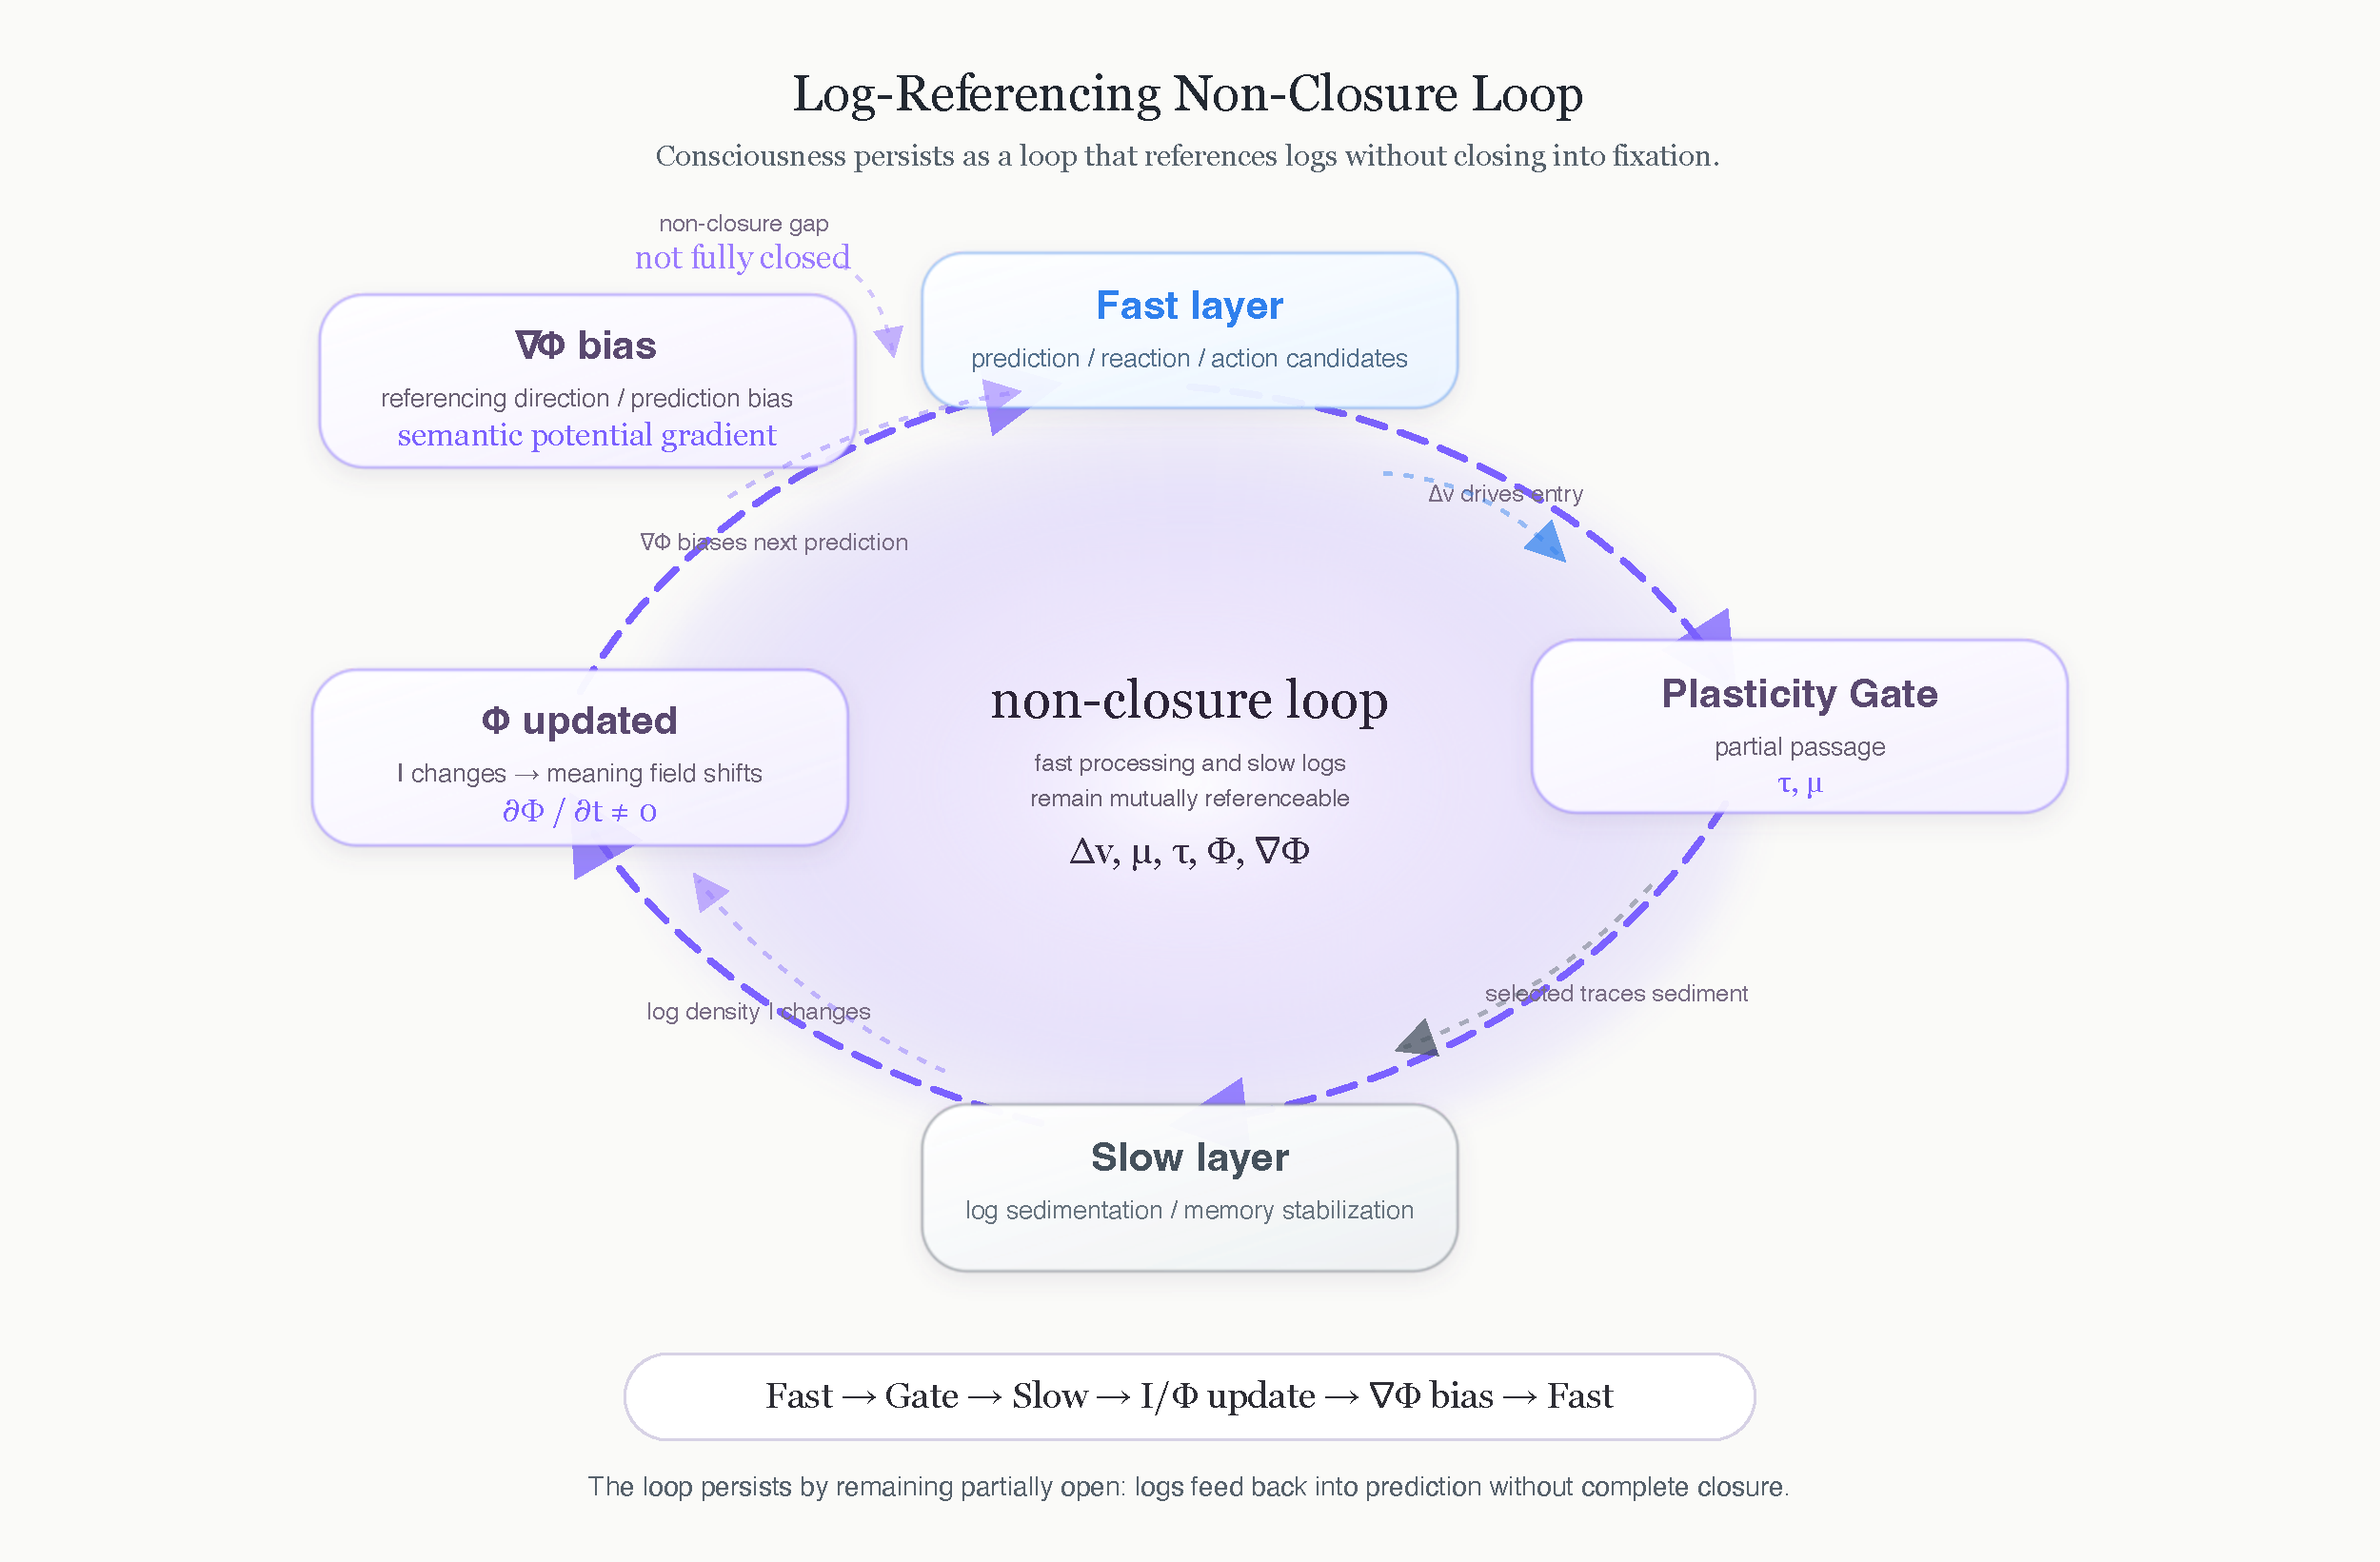
\includegraphics[width=0.92\linewidth]{figures/figure4_log_referencing_loop.pdf}
\caption{
Log-referencing non-closure loop.
Fast processing passes partially through the plasticity gate into slow log sedimentation.
Changes in log density update the meaning potential, whose gradient biases subsequent prediction.
The loop persists by remaining partially open.
}
\label{fig:log-loop}
\end{figure}

Through this loop, the conscious state becomes not merely a momentary event but a structure sustained across time.

However, this loop does not close completely.

Complete closure would fix processing and eliminate plasticity.

Complete openness would prevent sedimentation and prevent log referencing from obtaining.

The log-referencing loop is therefore maintained in a non-closed form.

This non-closure is the condition for the persistence of the conscious state.

\subsection{Conscious Access and Report}


Conscious state and reportability are not identical.

However, in the framework of this paper, the two are closely related.

Report is the externalization of logs sedimented in the slow layer through language or action.

Processing that occurs but does not sediment into the slow layer cannot be reported.

What has sedimented but is not connected to reporting pathways cannot be explicitly articulated.

In Libet-type experiments, the problem concerns the time difference between action preparation and reportable timestamp.

In split-brain experiments, the problem concerns the spatial disconnection between processing and reporting pathways.

In both cases, the question is not whether consciousness exists but how processing connects to the pathways of log referencing and reportability.

\subsection{Non-Closure of the Loop}


The log-referencing loop is not better for being more stable.

Too stable, and it becomes fixed.

Too unstable, and it fragments.

What consciousness requires is therefore not a closed loop but a loop that does not close completely.

This structure corresponds to VED's non-closure principle.

There is difference; gradient forms; flow arises; structure tends toward closure — but does not close completely.

The conscious state is the same.

Current processing tends to sediment into logs.

Logs tend to constrain current processing.

The meaning field tends to direct referencing.

But nothing becomes completely fixed.

This uncompleted loop maintains the conscious state.

\subsection{Summary}


This section organized the dynamic process of log referencing.

Consciousness is understood as the non-closure loop formed by fast layer, slow layer, plasticity gate, internal delay, meaning gradient, and effective torque-like quantity.

In this loop:

\begin{itemize}
\item The fast layer anticipates the future.
\item The slow layer sediments the past.
\item The plasticity gate regulates what sediments.
\item Internal delay $\tau$ provides the temporal thickness of referencing.
\item Meaning gradient $\nabla\Phi$ biases the direction of referencing.
\item $\mathcal{T}_{\Phi}$ represents the referencing load coupling speed difference and meaning gradient.
\item Non-closure is the condition for the loop's persistence.
\end{itemize}

Consciousness is therefore not the storage of logs.

Nor is it the running of processing.

Consciousness is the state in which fast processing and slow logs become mutually referenceable, along the meaning gradient, within a loop that does not close completely.
